\section{Modifications to the cross-entropy loss for PU Learning}
\label{sec:pulearning}


%%%%%%%%%%%%%%%%%%%%%%%%%%%%%%%%%%%%%%%%%%%%%%%%%%%%%%%%%%%%%%%%%%%%%%
%%%%%%%% FIGURE Losses
%%%%%%%%%%%%%%%%%%%%%%%%%%%%%%%%%%%%%%%%%%%%%%%%%%%%%%%%%%%%%%%%%%%%%%

\begin{figure}[t]
\centering
% \fbox{\rule{0pt}{2in} \rule{0.9\linewidth}{0pt}}
   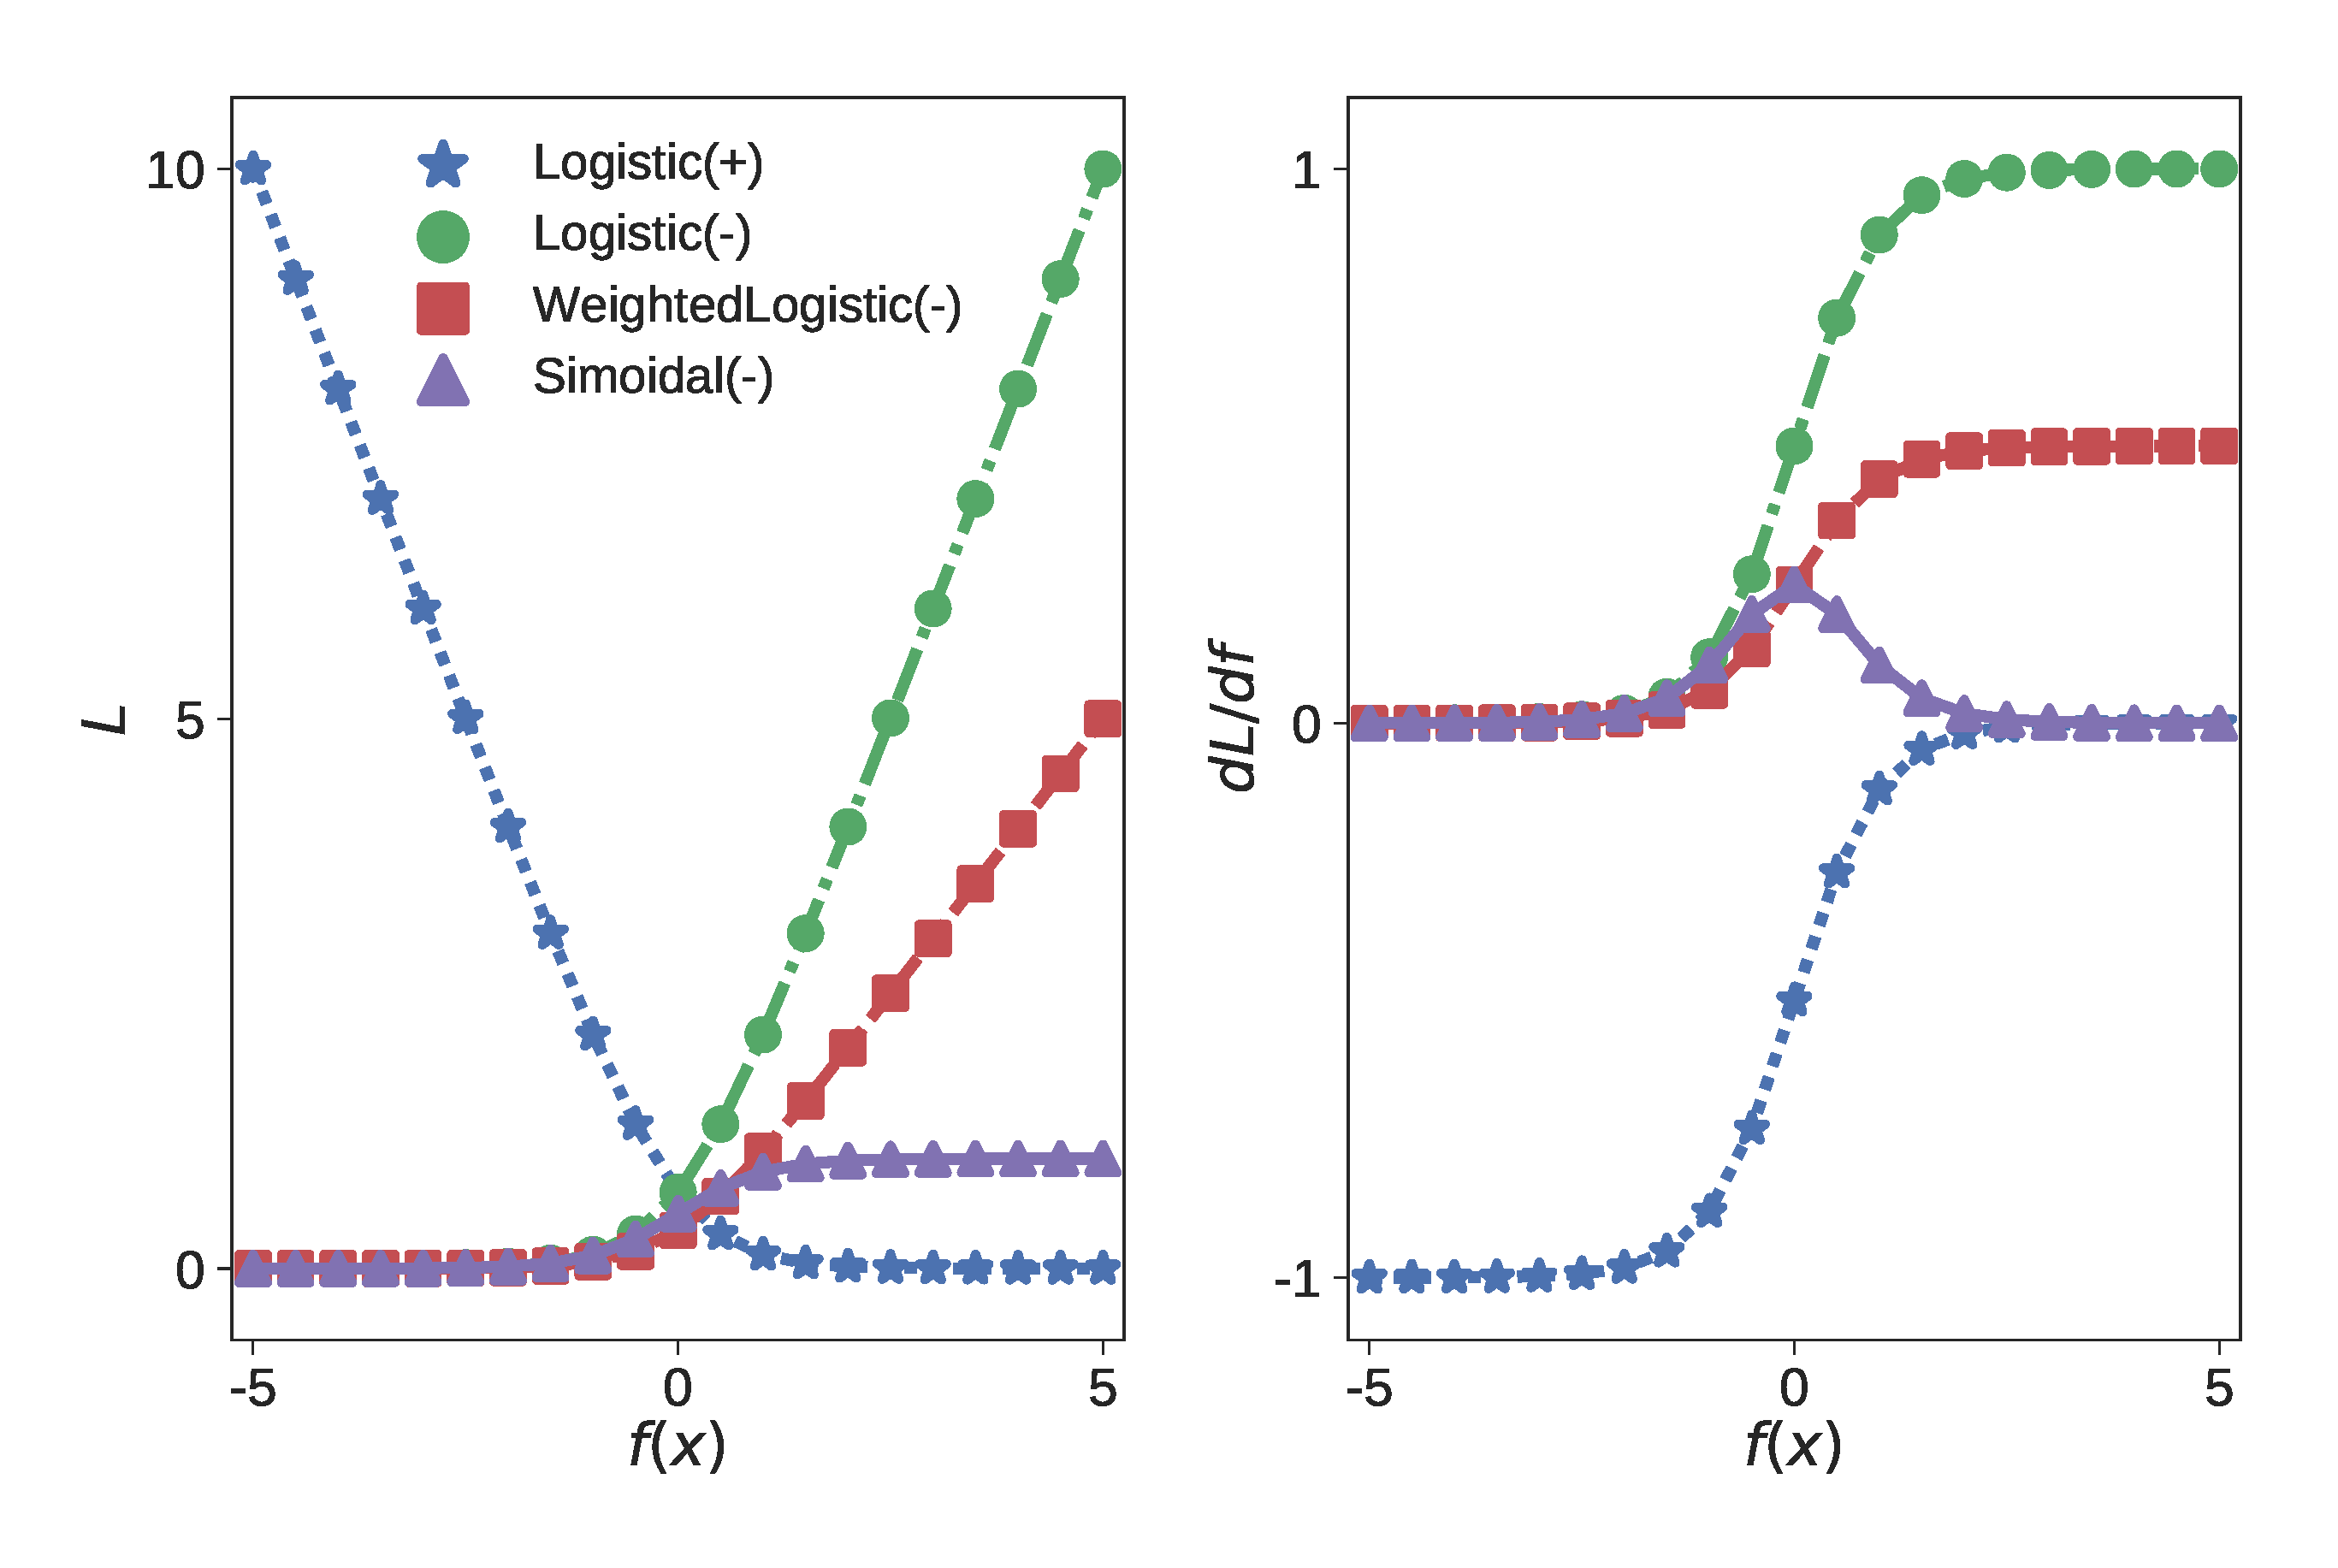
\includegraphics[width=1.05\linewidth]{img/losses}
\caption{
The differences in losses (top figure) and derivatives (bottom figure) with repect to logits between the weighted logistic negative loss and the sigmoidal negative loss.
The \textbf{+} sign represents the loss of positive samples and the \textbf{-} sign stands for the loss of negative samples.
The sigmoidal loss of negative examples reaches a plataeu and the derivative drops to zero in the very positive region, whereas the weighted logistic loss for negative is just a linearly scaled logistic loss.
}
\label{fig:losses}
\end{figure}

%%%%%%%%%%%%%%%%%%%%%%%%%%%%%%%%%%%%%%%%%%%%%%%%%%%%%%%%%%%%%%%%%%%%%%
%%%%%%%% TEXT PU Learning setup
%%%%%%%%%%%%%%%%%%%%%%%%%%%%%%%%%%%%%%%%%%%%%%%%%%%%%%%%%%%%%%%%%%%%%%

\paragraph{PU Learning}

A training set of the positive and negative (PU) learning problems contains only a set of positive examples (P set) and a set of unlabeled samples (U set).
Unlabeled examples can be either positive or negative, meaning that there is no reliable negative examples available
One straightforward way to generate negative examples for training is to treat all the unlabeled examples as a set of negative examples with noises.
The problem then converts to learning with clean positive labels and noisy negative labels.
The goal of solving a PU learning problem is to learn a classifier that predicts as many positives as possible while keeping the false positive rate low, regardless the influence of false negative labels.
In other words, the purpose is to achieve high recall without sacrificing too much precision.


%%%%%%%%%%%%%%%%%%%%%%%%%%%%%%%%%%%%%%%%%%%%%%%%%%%%%%%%%%%%%%%%%%%%%%
%%%%%%%% TEXT Weighted loss for negatives
%%%%%%%%%%%%%%%%%%%%%%%%%%%%%%%%%%%%%%%%%%%%%%%%%%%%%%%%%%%%%%%%%%%%%%

\paragraph{Weighted logistic loss for negative class}

The mislabeled negative samples bias the classifier to have low recall.
It is possible to balance precision and recall by simply weighing the positive and negative examples differently, namely, let the positive and negative examples have different rates of contribution to the total loss.
Suppose a logistic loss is used, the corresponding weighted loss for a input-output pair $(x, y)$ for a classifier determined by parameters $\theta$ is:
\[
  l(x, y; \theta) =
    \begin{cases}
      - \alpha \log P(y=+1 \vert x; \theta), & y = +1 \\
      - \beta \log P(y=-1 \vert x; \theta), & y = -1
    \end{cases}
\]
where $\alpha$ and $\beta$ are weights for positive and negative class respectively, and $P(y\vert x; \theta)=\sigma(f(x; \theta))$ is the probablistic predictions by model $f(\cdot)$, activated by the sigmoid function $\sigma(\cdot)$.
This loss is referred to as the \textbf{weighted loss} in the rest of paper.
Empirically, the choice of $p$, $q$ can be made based on the highest precision and recall achieved on a validation set, or alternatively based on a class priors estimation\cite{du2014class}.
% Alternatively, one can also roughly assign $q=p(y=-1 \vert \tilde{y}=-1)$.
% This turns out to be part of the backward corrected loss proposed in  \cite{patrini2016making}:
% \begin{equation*}
%   \begin{aligned}
%     l_{\tilde{y_i}=-1} = - p(y_i=-1 \vert \tilde{y_i}=-1) \log p(y_i=-1 \vert x_i) \\ - p(y_i=+1 \vert \tilde{y_i}=-1) \log p(y_i=+1 \vert x_i)
%   \end{aligned}
% \end{equation*}
% % $$p( \tilde{y} \vert x, y) = \sum_{y}p(\tilde{y} \vert y)p(y \vert x)$$
% % $$p(y=+1 \vert \tilde{y}=+1) = 1 $$
% % $$p(y=-1 \vert \tilde{y}=+1) = 0 $$
% with $p(y_i=-1 \vert \tilde{y_i}=-1) = q$ and $p(y_i=+1 \vert \tilde{y_i}=-1) = 1-q$.



%%%%%%%% TEXT Sigmoidal Negative loss
\paragraph{Sigmoidal Loss for negative class}

As motivated in Section \ref{sec:related}, we used a class-dependent loss to down-weight the loss contribution of very positive predictions negative labels and still making full use of the clean positive labels.
The loss of positive examples is still a normal logistic loss and the loss of negative examples is replaced with a sigmoidal loss \cite{tax2016class}:
\[
  l(x, y; \theta) =
    \begin{cases}
      - \alpha \log P(y=+1 \vert x; \theta), & y = +1 \\
      - \beta (1 - P(y=-1 \vert x; \theta)), & y = -1
    \end{cases}
\]
We called this class-dependent loss \textbf{sigmoidal loss} in a sense it uses a sigmoidal function as the loss of negative samples.

Figure \ref{fig:losses} shows the differences in losses and derivatives with respect to model output between weighted logistic loss and sigmoidal loss.
The main feature of sigmoidal loss for negative examples is its small changes in the region of confident positive, compared to the weighted loss with $\alpha=1$ and $\beta=0.5$.
As a consequence, the corresponding derivative decreases to zero as the model prediction increases in the positive direction.


%%%%%%%% TEXT Bootstrapping
\paragraph{Hard bootstrapping loss for negative class}
In addition to the proposed sigmoidal loss, we also modify the hard bootstrapping loss by Reed et al. \cite{reed2014training} for PU learning to set a benchmark.
The modified class-dependent hard bootstrapping loss a pair of inputs and label $(x,y)$ is:
% $$l_- = - \beta \log p(y=-1 \vert x) - (1-\beta) \sum_{j\in \{-1, +1\}} p(y=j \vert x) \log p(y=j \vert x)$$
\begin{equation*}
\resizebox{\columnwidth}{!}{$
  l(x, y; \theta) =
    \begin{cases}
      - \log P(y=+1 \vert x; \theta), & y = +1 \\
      - \beta \log P(y=-1 \vert x;\theta) - (1-\beta) \log P(y=\hat{y} \vert x;\theta), & y = -1
    \end{cases}
$}
\end{equation*}
where $\hat{y} = \argmax_{j\in\{-1,+1\}}{P(y=j \vert x)}$ is the class with the highest predicted probability and $0<\beta<1$.
The first term of the objective is a weighted logistic loss and the second term can be considered as a regularization term to encourage consistent predictions.
This loss is referred as \textbf{bootstrapping loss} for the rest of this paper.
% \begin{equation*}
%   \begin{aligned}
%     H = - \sum_{j\in\{-1,+1\}} p(y_i=j \vert x_i) \log p(y_i=j \vert x_i) \\
%     \sim - \sum_{j\in\{-1,+1\}} \delta(y_i - \hat{y_i}) \log p(y_i=j \vert x_i)
%   \end{aligned}
% \end{equation*}
% which intuitively encourages the model to make confident predictions \cite{grandvalet2005semi}.

%%%%%%%% TEXT Multiple classes
\paragraph{Extend PU learning to multiclass problems}

For classification problems with multiple positive classes and one negative class, the weighted negative loss, sigmoidal negative loss and bootstrapping negative loss can be extended to train deep learning models in the presence of negatively labeled examples from various positive classes.
The logistic loss naturally extends to the multi-class scenario as the sigmoid activation extends to the softmax function.
Similar modifications can be then made to the cross-entropy loss, namely, keeping the losses for positive classes unchanged and applying the modifications to the loss for the negative class.
We used the manner of extending the losses in this work.
Alternatively, one can apply a one-vs-all strategy, with which the normal logistic loss is used for positive classes while the weighted, sigmoidal and bootstrapping loss can be used for the negative class.

%%%%%%%% TEXT Segmentation
\paragraph{Extend PU learning to segmentation}

By assuming the probability of missing positive label for a pixel is independent of its neighbor pixels, the weighted negative loss, sigmoidal negative loss and bootstrapping negative loss are all applicable to per-pixel classification problems if classification for each pixel is made independently.

% It is nevertheless difficult to fit such a NNAR model directly because it is difficult to estimate of $p(e \vert x,y)$ with limited number of samples.
% An alternatie model is the \textit{noisy at random (NAR)} model in which the occurence of errors $e$ are independent to $x$ only on $y$: $p(\tilde{y} \vert y)p(y \vert x)$
% Such \textit{Noisy at random (NAR)}

%%%%%%%% TEXT Expontial loss FADE IN
\paragraph{Implementation details}

We introduced the sigmoidal negative loss after training with a class-weighted cross entropy loss for a few epochs.
The sigmoidal loss of negative examples saturates for very positive outputs, meaning that the confident, positive prediction has little contribution to the weights update.
The wrong confident predictions can introduce problems at the beginning of the training procedure when the confident predictions are likely to be made at random.
Otimization would reach the plateau when the model made all positive predictions with high confidence.
Besides, we also introduce the modified hard bootstrapping loss only after a few epochs trained with class-weighted loss because it also relies on a nonrandom model for sufficiently reliable prediction $\hat{y}$.


%%%%%%%% TEXT Imbalanced

Another problem encountered in the PU learning setup is the class imbalance introduced by negatively labeled positive samples.
A balanced dataset can become imbalanced in the presence of false negative labels, especially if only a small portion of positive samples are correctly labeled.
We reweighed positive and negative samples based on their occurrences of the observed labels to alleviate the influence of imbalance for training.
Note that the class-weighted logistic loss reweighed the classes in addition to this frequency balancing class weight.
